\chapter{Quantum-Network Telescopes}
\label{chap:e24}

\begin{chapteropening}
In Chapter \ref{chap:e09} we learned to combine the light of two telescopes and count fringes: the fringe visibility is the complex visibility \(V\), and \(V\) encodes the angular structure of the star. But that chapter also left us with a heavy footnote: to keep the fringes stable, the optical path difference between the two arms must be locked to a precision far smaller than one wavelength, and any loss along either arm \emph{directly devours the already scarce starlight photons}. Stretch the baseline to a few kilometers, or a few tens of kilometers, and both requirements spiral out of control. This chapter asks a bold question: can we avoid \emph{hauling the unknown starlight over long distances} and yet still ``join'' two widely separated telescopes into a single instrument? The answer comes from quantum information: an \textbf{entanglement resource} that is prepared in advance, can be verified, and can be redone if it fails, together with \textbf{quantum memory} and a \textbf{quantum repeater}, lets the two ends ``share'' the phase relation of a single photon without forcing that fragile starlight photon to make the whole journey itself. This route is not yet a mature instrument but a feasibility ledger that must be worked out line by line; this chapter builds that ledger from the ground up and places it side by side with the intensity interferometry of Chapter \ref{chap:e10}.
\end{chapteropening}

\section{Why long-baseline amplitude interferometry is throttled by photon loss}
\label{sec:e24-why-loss}

Let us strip the problem down to its essence. What we really want to preserve is not ``more light'' but \emph{the phase of first-order coherence}. Imagine a point source in the sky; within one coherence time \(\tau_c\simeq1/\Delta\nu\) (Chapter \ref{chap:e02}) a single photon from it happens to fly to the telescope array. The key fact about extremely faint starlight is this: the mean number of photons from the object per time window, \(\epsilon\ll1\), is tiny: the vast majority of windows are empty, and now and then a single window contains just one photon. This one photon, if it has not been contaminated by any ``which-path'' information before reaching the detector, is \emph{not} a classical particle that ``already belongs to the left telescope'' or ``already belongs to the right telescope''; it is a quantum superposition of the left and right receiving paths:

\begin{equation}
  |\psi_\star\rangle
  =
  \frac{|1\rangle_L|0\rangle_R
  +
  e^{i\phi}\,|0\rangle_L|1\rangle_R}{\sqrt2},
  \qquad
  \phi=\frac{2\pi\,\bm{B}\cdot\bm{\theta}}{\lambda}.
  \label{eq:e24-stellar-single-photon}
\end{equation}
\begin{formulaexplain}
\(|\psi_\star\rangle\) is the path-superposition state of one starlight photon between the left and right apertures; \(|1\rangle_L|0\rangle_R\) means ``one photon on the left, nothing on the right,'' and the other term is the reverse. \(\phi\) is the geometric phase fixed by the baseline \(\bm{B}\), the source angular position \(\bm{\theta}\), and the wavelength \(\lambda\). What amplitude interferometry must preserve is precisely this \(\phi\).
\end{formulaexplain}

Here \(|1\rangle_L|0\rangle_R\) is number-state notation (Chapter \ref{chap:e05}): the subscripts \(L,R\) label the left and right spatial modes, and the numbers in the kets are the photon numbers in those modes. \(\bm{B}\) is the projected baseline (in cm, ranging in magnitude from \(10^2\,\mathrm{cm}\) to \(10^7\,\mathrm{cm}\)), \(\bm{\theta}\) is the angular position of the point source relative to the phase center (dimensionless radians), and \(\lambda\) is the wavelength (visible light \(\sim6\times10^{-5}\,\mathrm{cm}\)). The phase \(\phi\) is dimensionless and purely geometric: it is exactly the phase in the fringes of Chapter \ref{chap:e09}, only now written in the language of a single-photon superposition state.

A real star is not a point but a sum of many mutually incoherent point sources (this is precisely the starting point of the van Cittert--Zernike theorem in Chapter \ref{chap:e10}). Each subsource \(j\) gives its own pure state \eqref{eq:e24-stellar-single-photon} with phase \(\phi_j\); the incoherent superposition weights these pure states by brightness and sums them into a mixed state. After summation, what appears in the off-diagonal element is exactly the brightness-weighted average of those phase factors \(\langle e^{i(\phi_j-\phi_k)}\rangle\), which converges to precisely the complex visibility \(V\) of Chapter \ref{chap:e10}. Restricting to the single-photon subspace \(\{|10\rangle,|01\rangle\}\), the density matrix is

\begin{equation}
  \rho_1
  =
  \frac{1}{2}
  \begin{pmatrix}
  1 & V\\[2pt]
  V^* & 1
  \end{pmatrix}_{\{|10\rangle,\,|01\rangle\}} ,
  \qquad
  V=|V|\,e^{i\arg V}.
  \label{eq:e24-single-photon-density}
\end{equation}
\begin{formulaexplain}
\(\rho_1\) is the density matrix of the single-photon subspace; the diagonal elements \(\tfrac12\) only say ``the photon can appear at either telescope,'' while the off-diagonal element \(V\) is the complex visibility, carrying the coherent phase and angular structure of the source. \(|V|\) falls from 1 (a point source) to 0 (a source large enough to be resolved out), and the phase gives the source's position and asymmetry.
\end{formulaexplain}

Compare this with Eq.\ \eqref{eq:e10-gamma12} of Chapter \ref{chap:e10}: there the complex visibility \(\gamma^{(1)}_{12}\) is defined via the time average of the two field arms; the \(V\) here is the very same quantity, merely relocated to the off-diagonal element of the single-photon density matrix. The physical meaning is identical: \emph{to measure \(V\) is to measure the star}. The traditional amplitude-interferometry approach sends the two spatial modes \(L,R\) through fibers or free-space optical paths to \emph{the same} beamsplitter, turning \(\phi\) into countable fringes. The trouble lies precisely in this ``send to the same beamsplitter'' step: if one arm travels a lossy link of length \(L\), the single-photon transmittance is

\begin{equation}
  \eta_{\rm ch}(L)=10^{-\alpha_{\rm dB}L/10}.
  \label{eq:e24-link-loss}
\end{equation}
\begin{formulaexplain}
\(\eta_{\rm ch}\) is the link transmittance (dimensionless, \(0\) to \(1\)); \(\alpha_{\rm dB}\) is the loss in decibels per kilometer (units \(\mathrm{dB\,km^{-1}}\)), and \(L\) is the link length (km). The decibel loss makes the transmittance decay \emph{exponentially} with distance: this is the core bottleneck of direct optical combination over long baselines.
\end{formulaexplain}

The decibel is a logarithmic scale: \(10\,\mathrm{dB}\) means attenuation to \(1/10\), and \(20\,\mathrm{dB}\) means \(1/100\). Plug in real numbers to get a feel. Visible light in ordinary fiber suffers losses as high as \(20\)--\(30\,\mathrm{dB\,km^{-1}}\); over \(1\,\mathrm{km}\) only \(10^{-2}\) to below \(10^{-3}\) survives, and the starlight, already at \(\epsilon\ll1\), is nearly wiped out. Switch to the \(1550\,\mathrm{nm}\) telecom band, and the best fibers reach \(\sim0.2\,\mathrm{dB\,km^{-1}}\); but starlight does not naturally live in this band, so one must first do frequency conversion, coupling, and phase stabilization, each step multiplying in another sub-unity efficiency. A clear-sky free-space link can be taken as \(\sim0.5\,\mathrm{dB\,km^{-1}}\) for order-of-magnitude estimates, but the losses from atmospheric turbulence and pointing errors do not follow this clean exponential law \citep{2012PhRvL.109g0503G,2019PhRvL.123g0504K,2024SPIE13095E..1NR}. In a word: \emph{the more you want to lengthen the baseline, the farther you must send this already scarce starlight photon, and the probability of losing it rises exponentially with distance}.

\begin{figure}[tbp]
\centering
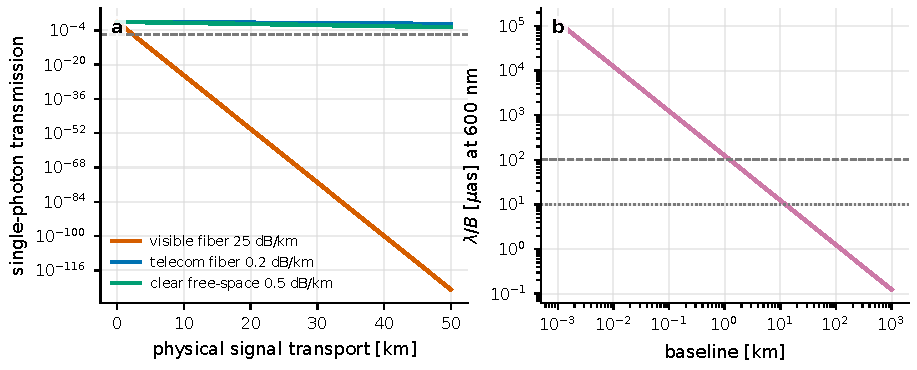
\includegraphics[width=0.94\linewidth]{figures/generated/chapter_17/ch17_architecture_loss.pdf}
\caption{The allure and the difficulty of long baselines come from the same dimension. The left panel plots the link loss for several ways of ``directly transmitting single-photon starlight'' as transmittance: visible-light fiber is already severely attenuated on kilometer scales, and even telecom-band fiber becomes expensive at hundred-kilometer scales. The right panel gives the angular-resolution scale \(\lambda/B\): \(600\,\mathrm{nm}\) light on a \(1\,\mathrm{km}\) baseline reaches the hundred-microarcsecond level, and a \(100\,\mathrm{km}\) baseline enters the microarcsecond regime.}
\label{fig:e24-architecture-loss}
\end{figure}

So why go to such lengths to stretch the baseline? Because the fundamental scale of angular resolution recognizes only the baseline length \(B\):

\begin{equation}
  \theta_{\rm res}\sim\frac{\lambda}{B}
  =124\,\mu\mathrm{as}
  \left(\frac{\lambda}{600\,\mathrm{nm}}\right)
  \left(\frac{1\,\mathrm{km}}{B}\right).
  \label{eq:e24-resolution-scale}
\end{equation}
\begin{formulaexplain}
\(\theta_{\rm res}\) is the angular-resolution scale of the interferometer (here in microarcseconds \(\mu\mathrm{as}\)), and \(B\) is the baseline length. The longer the baseline, the finer the angular structure that can be resolved. What the quantum-network scheme pursues is precisely pushing \(B\) to kilometers and beyond \emph{without hauling unknown starlight over long distances}.
\end{formulaexplain}

Set the ratios in the parentheses to 1 and you read off the benchmark of \(124\,\mu\mathrm{as}\); \(B=10\,\mathrm{km}\) gives \(12\,\mu\mathrm{as}\), and \(B=100\,\mathrm{km}\) gives \(1.2\,\mu\mathrm{as}\). For reference, the largest optical interferometric arrays (such as CHARA) have baselines of a few hundred meters and reach only the milliarcsecond level. The appeal of the quantum-network telescope is locked to this scale: it may not improve the sensitivity of a single aperture, but it could push optical/near-infrared interferometry from a few hundred meters all the way to kilometers, tens of kilometers, or longer. Intensity interferometry (HBT) of Chapter \ref{chap:e10} in fact already sidestepped the hurdle of optical-path transport: it does not combine beams but records intensity fluctuations locally and correlates them offline, and so is almost immune to atmospheric jitter, at the price of giving mainly \(|V|^2\) and losing the phase. The ambition of the quantum-network route is different: it wants to \emph{preserve the phase of first-order coherence} while \emph{not hauling unknown starlight over long distances}.

\section{Pre-shared entanglement: replacing what must be transported}
\label{sec:e24-gjc}

The central trick was devised by Gottesman--Jennewein--Croke: since hauling the fragile, unknown starlight over long distances is so costly, \emph{don't haul it}; instead, transport a ``laboratory photon'' that we fully control, can verify, and can remake if it breaks. This laboratory photon is prepared in advance in a known path-entangled state:

\begin{equation}
  |\Phi_\delta\rangle
  =
  \frac{|1\rangle_L|0\rangle_R
  +
  e^{i\delta}\,|0\rangle_L|1\rangle_R}{\sqrt2}.
  \label{eq:e24-lab-entangled-photon}
\end{equation}
\begin{formulaexplain}
\(|\Phi_\delta\rangle\) is the pre-shared laboratory path-entangled photon; its form is identical to the starlight state \eqref{eq:e24-stellar-single-photon}, except that the phase \(\delta\) is entirely under our control. It takes over the task of ``hauling unknown starlight over long distances'': this entanglement can be distributed in advance and verified afterward, and if it fails it is simply discarded and redone, never touching the precious starlight.
\end{formulaexplain}

Notice how strikingly similar the structures of \(|\Phi_\delta\rangle\) and \(|\psi_\star\rangle\) are: both are superpositions of ``one on the left / one on the right,'' differing only in that one phase is the heaven-set \(\phi\) and the other the human-set \(\delta\). This is the whole trick: let the \emph{known} \(\delta\) interfere locally with the \emph{unknown} \(\phi\), thereby reading out \(\phi\) (that is, \(V\)), while neither end has to send its own photon to the other.

How, concretely, do we read it? After the starlight photon arrives, each of the two stations \emph{locally} feeds its ``starlight mode'' and its ``laboratory entangled mode'' together into a beamsplitter, then keeps only certain \emph{coincidence} events, such as ``the left station detects one photon and the right station also detects one.'' The beamsplitter acts just as in Chapter \ref{chap:e09}: it linearly combines the two input amplitudes into the two output ports \((\text{starlight}\pm\text{laboratory})/\sqrt2\), so the field at each output is a \emph{coherent superposition} of the two path amplitudes. Once this is done, ``whether the photon was starlight or laboratory light, and which path it took'' is \emph{which-path information that gets erased}, leaving only the phase relation \(\phi-\delta\) between the two paths. The probability of a coincidence at both ends is proportional to the modulus squared of the coherently superposed amplitudes of these two erased paths; substituting the starlight state \eqref{eq:e24-stellar-single-photon} and the laboratory state \eqref{eq:e24-lab-entangled-photon} and expanding, the \emph{cross term} in the modulus squared is exactly \(\mathrm{Re}(V e^{-i\delta})\), and this is the carrier of the interference information. The full two-mode beamsplitter-plus-coincidence algebra is a standard result in quantum-optics textbooks; here we simply give its conclusion: the probabilities of the correlated and anti-correlated coincidence clicks are

\begin{equation}
  P_{\pm}(\delta)
  =
  \frac{1}{2}
  \Bigl[\,1\pm\mathrm{Re}\!\left(V\,e^{-i\delta}\right)\Bigr].
  \label{eq:e24-gjc-probability}
\end{equation}
\begin{formulaexplain}
\(P_\pm(\delta)\) are the probabilities of the two classes of coincidence clicks, \(V\) is the stellar complex visibility, and \(\delta\) is the laboratory phase that we can tune. Changing \(\delta\) is like scanning a reference phase: the click rate oscillates sinusoidally with \(\delta\), and from the amplitude and phase of the oscillation one reads out the real and imaginary parts of \(V\).
\end{formulaexplain}

Substituting \(V=|V|e^{i\arg V}\), we have \(\mathrm{Re}(Ve^{-i\delta})=|V|\cos(\arg V-\delta)\), so the \emph{oscillation depth} of \(P_\pm(\delta)\) as \(\delta\) varies is exactly \(|V|\), and its \emph{phase} is exactly \(\arg V\). In other words, sweeping \(\delta\) once measures the entire complex visibility, exactly the same physics as scanning the optical path difference to obtain fringes in Chapter \ref{chap:e09}, except that the reference phase is now provided by a local entanglement resource, and the starlight photon never leaves its own station from start to finish. This ``local beamsplitter + coincidence detection'' is called a \textbf{Bell-state measurement} in quantum information: it projects the two photons onto a basis of maximally entangled two-mode states. Unfortunately linear optics can unambiguously distinguish only some of the click combinations, so only about half of the usable starlight events enter the estimate; if one could perform a complete Bell-state measurement or more elaborate quantum processing, this \(50\%\) loss could in principle be avoided \citep{1982Natur.299..802W,1993PhRvL..70.1895B,2012PhRvL.109g0503G}.

A problem follows, and a hard one: the \textbf{resource rate}. This direct GJC route demands that \emph{every coherence-time window that might contain starlight have a matching entangled photon prepared in advance}. The bandwidth \(\Delta\nu\) sets the coherence time to about \(1/\Delta\nu\), so the number of time windows to cover per second is about \(\Delta\nu\). Take \(\Delta\nu=10\,\mathrm{GHz}\) and that is \(10^{10}\) windows per second, meaning you need a source that spits out \(10^{10}\) high-quality entangled photon pairs per second. Astronomical roadmaps (Rajagopal et al.) make it explicit that the best current entangled-photon sources fall far short of this rate; direct GJC is therefore better suited as a \emph{short-baseline in-sky proof of principle}, and in the near term it cannot yet replace existing optical interferometric arrays \citep{2024SPIE13095E..1NR,2012PhRvL.109g0503G}.

The scheme of Khabiboulline--Borregaard--De Greve--Lukin cleverly turns the very weakness of starlight to advantage. Since each long measurement window contains on average only \(\epsilon\ll1\) correlated starlight photons, one slices the window into \(M\sim1/\epsilon\) finer time bins, so that \emph{at most one bin} actually contains a photon. To record ``which bin the photon landed in,'' the clumsy way (a unary code, one bit per bin) needs \(M\) entangled pairs; the clever way (a binary code that encodes the arrival time in binary) needs only

\begin{equation}
  n_{\rm mem}
  =
  \bigl\lceil\log_2(M+1)\bigr\rceil
  \simeq
  \bigl\lceil\log_2(1/\epsilon)\bigr\rceil
  \label{eq:e24-binary-timebin}
\end{equation}
\begin{formulaexplain}
\(n_{\rm mem}\) is the number of storage qubits required, \(M\) is the number of time bins, and \(\epsilon\) is the mean number of starlight photons per bin. The \emph{sparsity} of faint light compresses the resource requirement from \(M\) entangled pairs down to about \(\log_2 M\) storage bits: an exponential saving.
\end{formulaexplain}

storage qubits, with each bit using one entangled pair to perform a nonlocal \textbf{parity check}. The scaling immediately becomes enticing: if \(M=10^6\), only about \(20\) qubits are needed to encode the arrival time, whereas a unary code would require a million entangled pairs. A representative worked example from the paper is: for a bandwidth \(\Delta f=1\,\mathrm{MHz}\) and a \(1\,\mathrm{s}\) measurement window, \(N=10^6\) time bins correspond to \(\log_2 N\simeq20\) qubits; in an astronomical example with a \(10\)th-magnitude star, \(10\,\mathrm{m^2}\) collecting area, and \(10\,\mathrm{GHz}\) detection bandwidth, the inferred resource target is roughly \(20\)--\(30\) qubits plus an entanglement-supply rate of \(\sim200\,\mathrm{kHz}\). A supplementary analysis by Stas et al.\ also uses \(20\) SiV nodes, a \(1\,\mathrm{kHz}\) zero-distance entanglement rate, and a \(1\,\mathrm{s}\) window to demonstrate a viable path toward this logarithmic scaling \citep{2019PhRvL.123g0504K,2022PhRvA.106c2424C,2026Natur.651..326S,2024SPIE13095E..1NR}.

\begin{figure}[tbp]
\centering
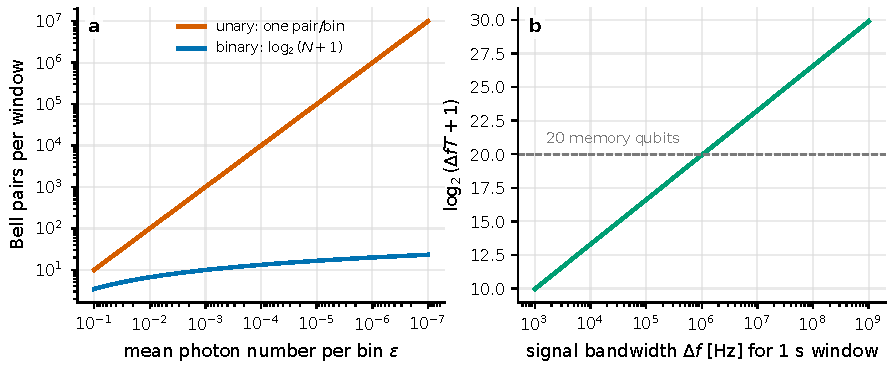
\includegraphics[width=0.94\linewidth]{figures/generated/chapter_17/ch17_timebin_scaling.pdf}
\caption{It is precisely because ``starlight is weak'' that time-bin encoding becomes meaningful. The left panel compares the entangled-pair requirements of unary versus binary encoding: when the mean photon number per bin \(\epsilon\) is small, \(M\sim1/\epsilon\) bins can be labeled with only \(\log_2(M+1)\) storage qubits. The right panel shows that in a \(1\,\mathrm{s}\) measurement window, a \(1\,\mathrm{MHz}\) bandwidth corresponds to about \(10^6\) bins, that is, about \(20\) qubits.}
\label{fig:e24-timebin}
\end{figure}

The underlying communication technology that supports all of this is the \textbf{quantum repeater}. Why can we not amplify a quantum state and send it far, the way we boost an electrical signal? Because the \emph{no-cloning theorem} forbids perfectly copying an unknown quantum state \citep{1982Natur.299..802W}, while loss rises exponentially with distance (Eq.\ \eqref{eq:e24-link-loss}). The repeater's idea is divide and conquer: cut the long distance into many short segments, first establish entanglement within each short segment (short segments have small loss and high success probability), then use \textbf{entanglement swapping} to ``relay'' the entanglement of adjacent segments into entanglement spanning the whole distance. An ideal repeater can trade exponential loss for much gentler resource scaling, but a real system must still face a chain of penalties: the success probability of the Bell-state measurement, the storage lifetime, dark counts, gate fidelity, and frequency conversion. The DLCZ atomic-ensemble protocol, quantum-internet roadmaps, and quantum-memory reviews all place \emph{storage} squarely at the center of the resource budget, because the job of storage is to \emph{align in time} these probabilistically successful events \citep{1998PhRvL..81.5932B,2001Natur.414..413D,2011RvMP...83...33S,2008Natur.453.1023K,2012IEEEN..26d..59V,2006quant.ph..7182U}.

\section{The resource ledger: how entanglement rate, storage time, and fidelity close together}
\label{sec:e24-budget}

Whichever of the above schemes we choose, in the end all return to the same ledger. Angular resolution is handed to us for free by \(B\) (Eq.\ \eqref{eq:e24-resolution-scale}), but \emph{whether an observation is actually possible} requires the entanglement-supply rate, the storage time, the fidelity, and the starlight event rate to all meet their targets \emph{simultaneously}; if even one falls short, the phase lever of the long baseline cannot be pried loose.

The first item is the \textbf{entanglement-supply rate}. Let the accepted effective starlight event rate be \(R_\star\), and let each event consume on average \(n_{\rm pair}\) entangled pairs; then

\begin{equation}
  R_{\rm ent}
  \gtrsim
  \frac{n_{\rm pair}\,R_\star}{p_{\rm ready}} .
  \label{eq:e24-entanglement-rate}
\end{equation}
\begin{formulaexplain}
\(R_{\rm ent}\) is the required entanglement-supply rate (units Hz), \(R_\star\) is the effective starlight event rate (Hz), \(n_{\rm pair}\) is the number of entangled pairs consumed per event, and \(p_{\rm ready}\) is the probability that an entangled pair is ready when the starlight arrives. It \emph{directly translates} the astronomical event rate into a throughput requirement on the quantum network.
\end{formulaexplain}

To understand this equation, one must first be clear about \(R_\star\): it is \emph{not} the total photon rate received by the telescope but the rate of events that entered the target spatial mode, frequency channel, and polarization channel, fell within the time window, and passed quality selection: the events \emph{actually usable}. The closer \(p_{\rm ready}\) is to 1, the more the entanglement resource is essentially always on standby, and the less is wasted. The lesson of this equation is direct: for a bright, broadband source, \(R_\star\) is enormous, and direct GJC is crushed by the resource rate; for a narrowband, faint source, \(R_\star\) is small, and only then does a storage-assisted scheme have a chance to trade a lower \(R_{\rm ent}\) for a long baseline.

The second item is the \textbf{storage time}. At the very least, the quantum state or measurement record must be kept until the classical communication and the nonlocal check are both complete:

\begin{equation}
  T_{\rm mem}
  \gtrsim
  \max\!\left[\frac{B}{c},\,T_{\rm ent},\,T_{\rm proc},\,T_{\rm win}\right].
  \label{eq:e24-memory-time}
\end{equation}
\begin{formulaexplain}
\(T_{\rm mem}\) is the minimum time for which the quantum memory must remain coherent, equal to the maximum of the four terms on the right: the baseline light-travel time \(B/c\), the entanglement-generation time \(T_{\rm ent}\), the processing time \(T_{\rm proc}\), and the measurement window \(T_{\rm win}\). The real bottleneck is often \emph{not} \(B/c\) but synchronization and the time-bin window.
\end{formulaexplain}

Plug in numbers and it becomes clear: the light-travel time \(B/c=3.3\,\mu\mathrm{s}\times(B/\mathrm{km})\), so a \(100\,\mathrm{km}\) baseline needs only \(0.33\,\mathrm{ms}\) of light-travel time, which sounds easy. But the Khabiboulline-type binary time-bin scheme, in order to cover narrowband faint light, may need a measurement window \(T_{\rm win}\) as long as \(\sim1\,\mathrm{s}\), several orders of magnitude more demanding than the light-travel time. Quantum-memory hardware is usually described by six figures of merit: fidelity, efficiency, storage time, bandwidth, multimode capacity, and operating wavelength. For single-photon storage, the \emph{conditional fidelity} is the overlap between the retrieved wave packet and the written one, and the \emph{efficiency} is the probability of successfully retrieving the photon; once one wants to interfere the stored photon with starlight, the \emph{product} of these two, plus phase noise and mode matching, directly lowers the final visibility \citep{2009NaPho...3..706L,2010EPJD...58....1S,2016JMOp...63.2005H}.

\begin{figure}[tbp]
\centering
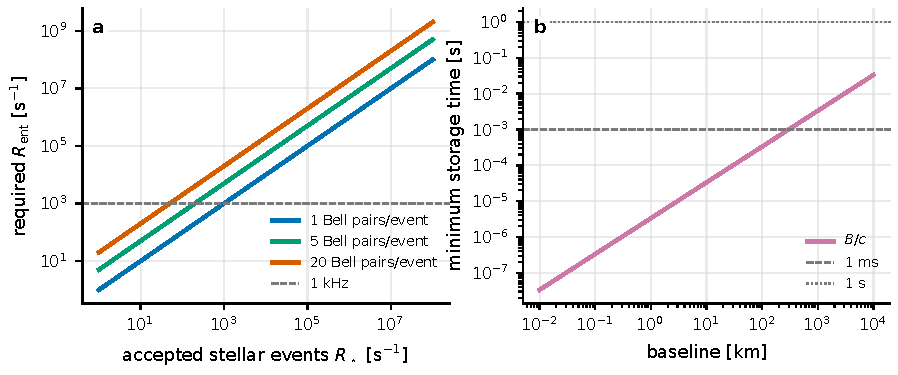
\includegraphics[width=0.94\linewidth]{figures/generated/chapter_17/ch17_entanglement_resources.pdf}
\caption{The entanglement rate and storage time give the first layer of resource-closure conditions. The left panel converts the accepted starlight event rate \(R_\star\) into the required entangled-pair rate: the more pairs each event consumes, the higher the demand line rises. The right panel converts the baseline into light-travel time \(B/c\): for kilometer-scale baselines, the light-travel time is only microseconds to milliseconds, but narrowband storage schemes are often dictated by the measurement window and the entanglement-generation time.}
\label{fig:e24-entanglement-resources}
\end{figure}

The third item is the \textbf{fidelity}. The resource budget often simply \emph{multiplies} several major penalty factors along the link to obtain a rough effective fidelity:

\begin{equation}
  F_{\rm eff}
  \simeq
  F_{\rm Bell}\,
  \eta_{\rm write}\,\eta_{\rm read}\,\eta_{\rm conv}\,
  e^{-T/T_2}\,
  (1-p_{\rm dark})\,
  M_{\rm mode}.
  \label{eq:e24-effective-fidelity}
\end{equation}
\begin{formulaexplain}
\(F_{\rm eff}\) is a rough effective resource quality, multiplying together the entangled-pair fidelity \(F_{\rm Bell}\), the write/read efficiencies, the frequency-conversion efficiency, the storage decoherence \(e^{-T/T_2}\), the dark-trigger term \((1-p_{\rm dark})\), and the mode matching \(M_{\rm mode}\). \emph{Any one factor being low lowers the final visibility multiplicatively}.
\end{formulaexplain}

Naming the units one by one: \(F_{\rm Bell}\) (dimensionless, \(\le1\)) is the fidelity of the pre-shared entangled pair; \(\eta_{\rm write},\eta_{\rm read}\) (dimensionless) are the write and read efficiencies; \(\eta_{\rm conv}\) is the frequency-conversion efficiency; \(T_2\) is the storage coherence time (units s), \(T\) is the actual storage duration; \(p_{\rm dark}\) is the equivalent dark-trigger probability; and \(M_{\rm mode}\le1\) denotes the degree of matching across the four types of mode: frequency, time, polarization, and space. This is not a complete quantum-channel model, but it has a virtue: it \emph{exposes the bottleneck at a glance}. Looking at the decoherence factor alone, \(T/T_2=1\) already gives a factor of \(e^{-1}\simeq0.37\); further assume \(F_{\rm Bell}=0.8\), read and write \(0.7\) each, and conversion \(0.8\) (not yet counting dark counts and mode mismatch), and multiplying, \(0.8\times0.7\times0.7\times0.8\simeq0.31\), the final visibility is already down to around thirty percent. This is why such schemes cannot fixate on ``how enticing the angular resolution is'' but must make every factor \emph{simultaneously} close.

\begin{figure}[tbp]
\centering
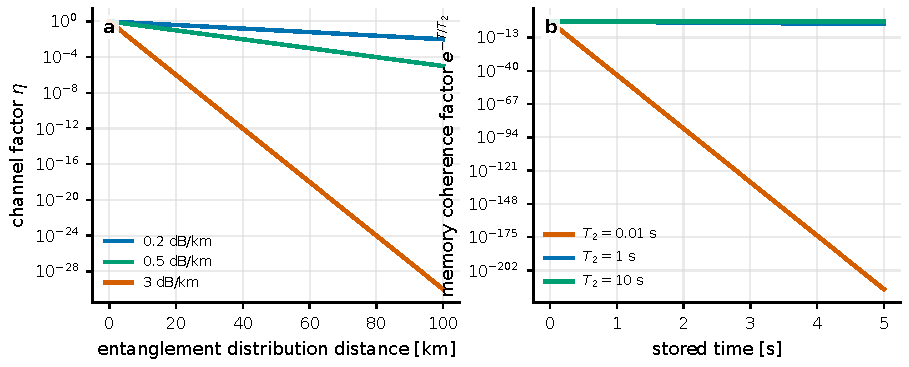
\includegraphics[width=0.94\linewidth]{figures/generated/chapter_17/ch17_fidelity_distance.pdf}
\caption{The effective resource quality is determined jointly by the link and the storage. The left panel gives the fall of the channel factor with distance for various \(\mathrm{dB\,km^{-1}}\) losses; the right panel gives the fall of the storage-decoherence factor \(e^{-T/T_2}\) with storage duration. However enticing its angular resolution, a long-baseline scheme must make the entangled-pair fidelity, the read/write efficiency, the frequency conversion, and the storage coherence all meet their targets \emph{together}.}
\label{fig:e24-fidelity-distance}
\end{figure}

Among these, \textbf{frequency conversion} is an extra difficulty specific to the astronomical version. Many quantum-memory materials couple strongly at frequencies that do not lie in the astronomical band we want to observe, while long-distance fiber prefers the telecom band, so one must do \emph{quantum frequency conversion}: change the photon's frequency while preserving its single-photon coherence, polarization, or time-bin encoding, and suppress the noise the conversion process introduces. Especially deadly is mode matching: if the post-conversion spectral width, center frequency, temporal wave packet, and polarization do not align with the starlight, then even a \(1\%\) mismatch loses \emph{not merely \(1\%\) of the photon count}: it is deducted directly from the interference visibility, because the visibility measures precisely ``how much alike'' the two beams are \citep{1990OptL...15.1476K,2010EPJD...58....1S,2016JMOp...63.2005H,2024SPIE13095E..1NR}.

\section{Continuous variables and ancilla single photons: what the other two routes each solve}
\label{sec:e24-cv-ancilla}

The schemes above all treat the ``left/right path'' as a discrete qubit and then stuff the timing information into storage. There are two more complementary ideas, and they solve different bottlenecks.

The first is the \textbf{continuous-variable} route. Here ``continuous variable'' refers to the two quadratures of the light field, the real and imaginary parts of the complex-amplitude arrow (Chapter \ref{chap:e01}), rather than an either/or discrete choice like ``left/right.'' Continuous-variable quantum teleportation uses a pre-shared \emph{two-mode squeezed vacuum} (TMSV) as its resource, transferring the quadrature information of one mode to a distant end via local measurement:

\begin{equation}
  |\psi_{\rm TMSV}\rangle
  =
  \sqrt{1-\lambda^2}\,
  \sum_{n=0}^{\infty}\lambda^n\,|n\rangle_A|n\rangle_B,
  \qquad
  \bar N=2\sinh^2 r .
  \label{eq:e24-tmsv}
\end{equation}
\begin{formulaexplain}
\(|\psi_{\rm TMSV}\rangle\) is the two-mode squeezed-vacuum resource state, with \(A,B\) the two widely separated modes; \(\lambda=\tanh r\) (with \(r\) the squeezing parameter) controls the squeezing strength, and \(\bar N\) is the total mean photon number. The stronger the squeezing, the smaller the added noise of continuous-variable teleportation, but the higher the resource cost.
\end{formulaexplain}

What this equation says is: the photon numbers of the \(A\) end and the \(B\) end \emph{are always equal} (both take the value \(n\)), and the amplitudes of different \(n\) are arrayed as \(\lambda^n\): this is precisely the quantum fingerprint of ``two modes squeezed together.'' The ideal case requires \(r\to\infty\) (infinitely strong squeezing) to transmit an arbitrary continuous-variable state noiselessly; in reality \(r\) is finite, so an equivalent Gaussian noise is mixed in, usually decaying as \(e^{-2r}\) as the squeezing strengthens. The continuous-variable teleportation protocol of Braunstein--Kimble, together with the analysis of Gottesman et al., shows that this route can \emph{sidestep} the \(50\%\) ceiling of the discrete Bell measurement; but the price is that continuous-variable repeaters are harder and high-fidelity squeezing over long distances is more delicate. The most recent optimality analyses further caution that, when comparing different resource states, one must account for the \emph{photon-number superselection rule}, locality, and a finite entanglement budget: the degree of squeezing is only one line in the ledger, not the whole of it \citep{1998PhRvL..80..869B,2012PhRvL.109g0503G,2025PhRvR...7d3278Z}.

The second is the \textbf{ancilla single-photon} route, whose advantage is that it \emph{does not rely on long-lived quantum memory}. The idea of Marchese--Kok is: measure the fragile starlight photon locally at the receiving end as early as possible, and instead send an ancilla single photon (``produced on the ground, remakeable if broken'') across the baseline, so the loss falls mainly on the \emph{remakeable} ground photon rather than the irreproducible starlight. For a small-angle position estimate, the relation between phase and angle and the achievable angular precision satisfy

\begin{equation}
  \phi=\frac{2\pi B\theta}{\lambda},
  \qquad
  \sigma_\theta
  \ge
  \frac{\lambda}{2\pi B}\,
  \frac{1}{\sqrt{N_{\rm ev}\,\mathcal F_\phi}} .
  \label{eq:e24-angle-fisher}
\end{equation}
\begin{formulaexplain}
The left equation is the conversion between the angular position \(\theta\) and the interference phase \(\phi\); the right equation is the lower bound on the angular error, where \(N_{\rm ev}\) is the number of effective events and \(\mathcal F_\phi\) is the phase Fisher information of a \emph{single event} (Chapter \ref{chap:e12}). The longer the baseline, the more events, and the higher the per-event information, the more precise the localization.
\end{formulaexplain}

The right equation is in fact the result of applying the Cramér--Rao lower bound \eqref{eq:e12-crb} of the Fisher information \eqref{eq:e12-fisher-def} of Chapter \ref{chap:e12} to phase estimation: the total information is the per-event information \(\mathcal F_\phi\) times the number of events \(N_{\rm ev}\), the error falls as \(1/\sqrt{N_{\rm ev}\mathcal F_\phi}\), and the prefactor \(\lambda/(2\pi B)\) is the geometric coefficient converting phase error into angular error: the larger \(B\), the smaller the angular error corresponding to the same phase error, and this is the lever of the long baseline. In a model with \(\lambda=628\,\mathrm{nm}\) and fiber attenuation length \(L_0=10\,\mathrm{km}\), Marchese--Kok obtain a localization scale of order ten-odd \(\mu\mathrm{as}\). Modak--Kok further pour cold water on it: the starlight-mode occupation \(\epsilon\ll1\) and ``just how indistinguishable the ancilla photon is from the starlight'' significantly change the payoff: if \(\epsilon\) falls from 1 to \(0.01\), the benefit of adding ancilla photons quickly weakens; if the mode indistinguishability is only \(96\%\), a three-photon scheme might still turn a profit, but continuing to pile on more photons does not necessarily keep improving things \citep{2023PhRvL.130p0801M,2025PhRvA.111d3701M}.

Padilla, Sajjad, Saif, and Guha push the problem to a more general multimode-imaging limit: first perform \emph{local spatial-mode sorting} at each receiving station (borrowing the SPADE-type techniques of Chapter \ref{chap:e12}), then use pre-shared entangled pairs to simulate a nonlocal beamsplitter or even a more general interferometric network. This reminds us that the long baseline is only part of the resource: the mode information within a single aperture, the prior on source structure, the array geometry, and the choice of measurement basis all change the Fisher information one can ultimately extract. For the angular separation of a binary pair: if one fixates only on the Rayleigh-scale \(\lambda/B\), one misses the advantage of local mode sorting at \emph{small separations}; if one chases only local super-resolution, one loses the phase lever of the long baseline. The two must be used together \citep{2026PhRvA.113a2608P,2025PhRvR...7d3278Z}.

\section{From experimental prototype to error budget}
\label{sec:e24-prototype}

The value of an experimental prototype is not merely to prove that ``two distant nodes can be entangled,'' but to fill in a \emph{measurable number for every line} of the resource ledger. The 2026 experiment of Stas et al.\ moved ``nonlocal phase measurement'' from the schematic onto the lab bench. They used two SiV diamond-nanocavity nodes, equipped with electron-spin and \({}^{29}\mathrm{Si}\) nuclear-spin storage: first generating a remote entangled pair, then letting weak signal light interact locally with the node, and filtering out vacuum events through \emph{photon erasure} and nonlocal nondestructive heralding. In the experiment the electron Bell state reached \(F=0.83(3)\); at an entanglement rate of \(13\,\mathrm{Hz}\) it had \(F\ge0.5\), and dropping to \(1.9\,\mathrm{Hz}\) gave \(F=0.79(3)\). In the full nonlocal phase measurement, heralding raised the visibility from \(0.031(18)\) ``without heralding'' to \(0.090(26)\); after inserting a \(1.55\,\mathrm{km}\) fiber baseline, the visibility of the nuclear-spin parity oscillation was \(0.11(4)\), while the entangled-pair fidelity remained above the threshold for verifiable entanglement, at about \(F=0.63(3)\) \citep{2026Natur.651..326S}. Although these numbers are still far from astronomically usable, they turn the abstract \(F_{\rm Bell}\), \(R_{\rm ent}\), and \(V_{\rm meas}\) of the previous section's ledger, for the first time, into quantities measurable on the bench.

The phase error of such experiments is determined jointly by the number of effective trials, the heralding success rate, and the measured phase-oscillation visibility. Written in terms of Fisher information:

\begin{equation}
  \mathcal I_\phi
  \simeq
  N_{\rm tr}\,p_{\rm succ}\,V_{\rm meas}^2,
  \qquad
  \mathrm{Var}(\hat\phi)\ge\mathcal I_\phi^{-1} .
  \label{eq:e24-fisher-visibility}
\end{equation}
\begin{formulaexplain}
\(\mathcal I_\phi\) is the total phase Fisher information, \(N_{\rm tr}\) is the number of trials, \(p_{\rm succ}\) is the heralding success probability, and \(V_{\rm meas}\) is the measured visibility. The visibility enters the information as its \emph{square}, so a little coherence loss markedly amplifies the phase error; the right equation is the corresponding Cramér--Rao lower bound.
\end{formulaexplain}

Here \(N_{\rm tr}\) is how many times the protocol was run (dimensionless), \(p_{\rm succ}\) is the probability that a trial is accepted, and \(V_{\rm meas}\) is the visibility of the phase oscillation. The square in \(V_{\rm meas}^2\) is the crux: if the visibility drops to \(1/3\), the information drops to \(1/9\). And \(p_{\rm succ}\) itself decomposes as

\begin{equation}
  p_{\rm succ}=\eta_{\rm erasure}\,\eta_{\rm herald}\,P(n_{\rm photon}\ge1),
  \label{eq:e24-psucc}
\end{equation}
\begin{formulaexplain}
\(p_{\rm succ}\) is the probability that a trial is accepted, given by the product of the photon-erasure efficiency \(\eta_{\rm erasure}\), the heralding-detection efficiency \(\eta_{\rm herald}\), and the probability \(P(n_{\rm photon}\ge1)\) of ``at least one photon arriving.'' Raising it \emph{cannot} be done by simply cranking up the light intensity.
\end{formulaexplain}

This equation hides a counterintuitive trap. You might think: ``the higher the success rate \(p_{\rm succ}\) the better, so just raise \(P(n_{\rm photon}\ge1)\): why not pour in more photons?'' But once the mean photon number goes up, \emph{multiphoton contamination} rises with it: a trial that mixes in two or more photons disrupts the interference and lowers \(V_{\rm meas}\). And \(V_{\rm meas}\) enters \(\mathcal I_\phi\) as a square, while \(p_{\rm succ}\) enters only linearly, so \(p_{\rm succ}\) rises a bit, \(V_{\rm meas}\) falls a bit, and the total Fisher information \(\mathcal I_\phi=N_{\rm tr}p_{\rm succ}V_{\rm meas}^2\) actually \emph{falls rather than rises}. This is why ``a high heralding success rate'' is not necessarily a good thing. Finally, convert the phase error into an angular error via Eq.\ \eqref{eq:e24-angle-fisher}: the longer \(B\), the smaller the \(\sigma_\theta\) corresponding to the same \(\sigma_\phi\), but a long baseline also drives up the overhead of entanglement distribution, the difficulty of phase locking, and the latency.

\begin{figure}[tbp]
\centering
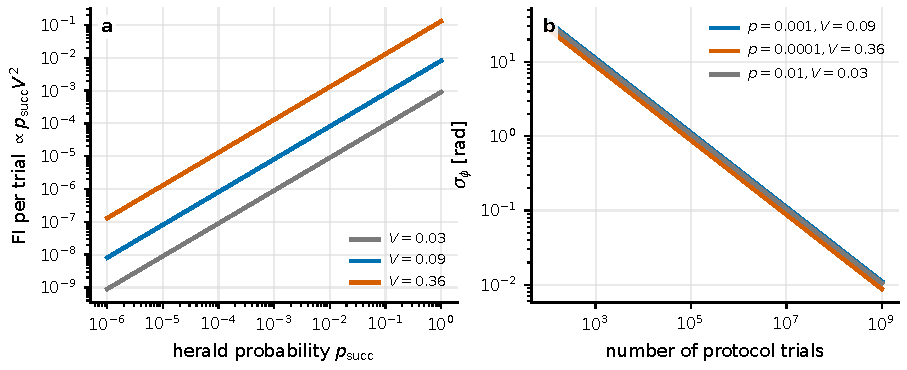
\includegraphics[width=0.94\linewidth]{figures/generated/chapter_17/ch17_fisher_visibility.pdf}
\caption{The statistical payoff of nonlocal phase measurement depends jointly on the success probability and the visibility. The left panel plots the single-trial Fisher-information scale \(p_{\rm succ}V^2\): a threefold drop in visibility gives a ninefold drop in information. The right panel converts the number of trials into phase error, showing that a high repetition rate, a low false-heralding rate, and a high entanglement fidelity must all hold \emph{simultaneously} before anything useful can be claimed.}
\label{fig:e24-fisher-visibility}
\end{figure}

The two-photon precision-astrometry experiment of Crawford et al.\ provides another near-term rung: using two pseudothermal light sources and time-tagging detectors, they observed in a tabletop mock-up the correlation behavior of photon-pair coincidences varying with phase. This experiment is not a complete quantum-network telescope, but it is very well suited as a \emph{rehearsal before going to sky}: time tagging, polarization matching, coherence time, HBT-peak fitting, phase stabilization, and data selection are all directly relevant to real astronomical faint-light observation \citep{2023OExpr..3144246C}.

Placing all the resources on one figure lets us see where we stand: near-term experiments sit roughly in the corner of \(R_{\rm ent}\sim1\)--\(10\,\mathrm{Hz}\), short baselines, and low effective visibility; whereas an astronomically usable ``storage-assisted narrowband'' scheme may need \(R_{\rm ent}\sim\mathrm{kHz}\) to \(100\,\mathrm{kHz}\), \(T_{\rm mem}\sim\mathrm{ms}\) to \(\mathrm{s}\), tens of storage qubits, and very high mode matching; broadband imaging is harder still. The four constraints must close \emph{together}: insufficient \(R_{\rm ent}\) wastes starlight events, insufficient \(T_{\rm mem}\) lets the parity check fall behind, insufficient \(F_{\rm eff}\) washes out the visibility, and if \(R_\star\) is once misestimated, the whole scheme may lose feasibility before the first night of observation.

\begin{figure}[tbp]
\centering
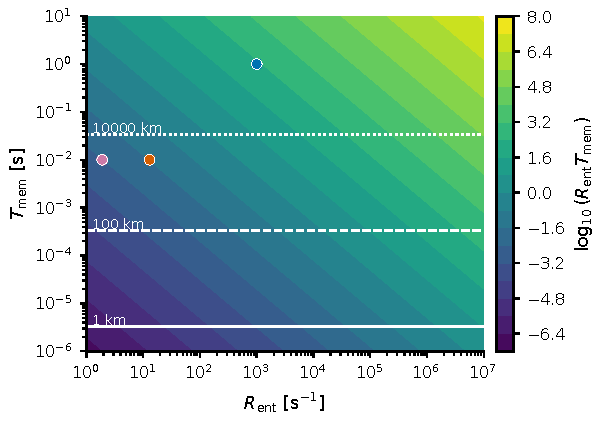
\includegraphics[width=0.94\linewidth]{figures/generated/chapter_17/ch17_network_parameter_space.pdf}
\caption{The resource space of the quantum-network telescope, spanned jointly by the entanglement rate and the storage time. White lines mark the \(B/c\) times corresponding to \(1\,\mathrm{km}\), \(100\,\mathrm{km}\), and \(10^4\,\mathrm{km}\) baselines; the scatter points give the order-of-magnitude gap between the Hz-level entanglement rates of current experiments and the far-term kHz--s-level targets. The color is only the scale of the resource product; full feasibility must be further multiplied by fidelity, mode matching, and the astronomical photon rate.}
\label{fig:e24-network-space}
\end{figure}

\section{How quantum networks and intensity interferometry complement each other}
\label{sec:e24-complementarity}

Please do not write the quantum-network telescope as something that ``replaces intensity interferometry'': it is a \emph{long-term complementary} route. Recall the division of labor between the two: the intensity interferometry of Chapter \ref{chap:e10}, relying on local time tagging plus offline correlation, long ago sidestepped optical-phase transport and is almost immune to atmospheric jitter, at the price of obtaining mainly \(|V|^2\) and losing the phase; the quantum-network route wants to \emph{preserve} the phase of first-order coherence, at the price of paying the whole ledger of entanglement, storage, frequency conversion, and heralding. In the near term, both must develop in parallel with the ELT, VLTI, CHARA, CTAO, and intensity-interferometry arrays.

A pragmatic phased roadmap goes as follows. The \emph{near-term} goal is intensity interferometry and two-photon correlation: the hardware is nearly off-the-shelf (large-area light collectors, SNSPD/SPAD time tagging, narrowband filtering, offline correlation), and the science goals center on the angular diameters of bright stars, binaries, and emission-line regions. The \emph{mid-term} adds local spatial-mode sorting, two-photon astrometry, and GJC-type short-baseline in-sky demonstrations, aiming to prove that the starlight mode can interfere \emph{stably} with a laboratory entanglement resource. Only in the \emph{far term} comes storage-assisted nonlocal first-order-coherence measurement, which requires quantum memory, frequency conversion, entanglement distribution, entanglement fidelity, and astronomical instrumentation to mature synchronously together \citep{1956Natur.178.1046H,2023OExpr..3144246C,2024SPIE13095E..1NR,2026Natur.651..326S}.

\Needspace{11\baselineskip}
Observation planning can start from a concise closure condition:

\begin{equation}
  N_{\rm useful}
  =
  R_\star\,T_{\rm obs}\,
  p_{\rm ready}\,p_{\rm succ}\,V_{\rm meas}^2
  \gtrsim
  N_{\rm req}(\sigma_\theta,\bm{B},\lambda) .
  \label{eq:e24-useful-events}
\end{equation}
\begin{formulaexplain}
\(N_{\rm useful}\) is the number of effective events that actually carry phase information, equal to the product of the starlight event rate, the observation time, the resource-ready probability, the success rate, and the visibility squared; \(N_{\rm req}\) is the number of events needed to reach the target angular precision \(\sigma_\theta\). Only when \(N_{\rm useful}\ge N_{\rm req}\) does the scheme have observational meaning.
\end{formulaexplain}

Naming the terms: \(T_{\rm obs}\) is the total observation time (s), and \(N_{\rm req}\) is set by the target angular precision, the array geometry, and the dimensionality of the model parameters. This equation puts astronomy and quantum engineering into \emph{one ledger}: a bright, narrowband signal with a known arrival time or period lowers the resource pressure, whereas a faint, broadband continuous source amplifies all the difficulties together. It is worth emphasizing that the same ledger applies to more general observation design as well, merely replacing the observable ``nonlocal phase'' with \(|V|^2\), \(g^{(2)}\), polarization angle, or time delay.

So the most valuable product of the quantum-network telescope for now is \emph{not} some already-built instrument but precisely this feasibility ledger that can be checked line by line. In the next chapter we return to the main line of observation design: mapping science goals onto event rates, channels, baselines, backgrounds, and covariances, and only then discussing the trade-offs among intensity interferometry, polarization event tables, transient triggers, and future nonlocal phase measurement.

\section*{Chapter Summary}
\addcontentsline{toc}{section}{Chapter Summary}

\begin{itemize}
\item \textbf{The source of the bottleneck.} Long-baseline amplitude interferometry must send scarce single starlight photons to the same beamsplitter, but the link loss rises \emph{exponentially} with distance (Eq.\ \eqref{eq:e24-link-loss}), while the longer the baseline the higher the resolution (Eq.\ \eqref{eq:e24-resolution-scale}): the allure and the difficulty come from the same dimension.
\item \textbf{Replace what must be transported.} Gottesman--Jennewein--Croke use a known, verifiable, remakeable pre-shared entangled photon \eqref{eq:e24-lab-entangled-photon} in place of hauling starlight over long distances; scanning the local phase \(\delta\) reads the complex visibility \(V\) from the coincidence click rate \eqref{eq:e24-gjc-probability}. The linear-optics Bell measurement incurs about a \(50\%\) event loss.
\item \textbf{The sparsity of faint light is a friend.} Each window contains on average only \(\epsilon\ll1\) starlight photons, so binary time-bin encoding compresses the resource from \(M\sim1/\epsilon\) entangled pairs down to about \(\log_2 M\) storage qubits (Eq.\ \eqref{eq:e24-binary-timebin}), and quantum repeaters and quantum memory take charge of aligning the probabilistically successful events.
\item \textbf{Four items must close together.} The entanglement-supply rate \eqref{eq:e24-entanglement-rate}, the storage time \eqref{eq:e24-memory-time}, the effective fidelity \eqref{eq:e24-effective-fidelity}, and the effective starlight event rate must all meet their targets simultaneously; the fidelity is a \emph{product} of factors, and any one falling short washes out the visibility multiplicatively. The mode mismatch of frequency conversion is especially deadly.
\item \textbf{Two more complementary routes.} Continuous-variable teleportation uses the two-mode squeezed vacuum \eqref{eq:e24-tmsv} to sidestep the \(50\%\) ceiling but with more delicate resources; the ancilla single-photon route \eqref{eq:e24-angle-fisher} lets a remakeable ground photon bear the link risk, but its payoff is sensitive to \(\epsilon\) and to mode indistinguishability.
\item \textbf{Visibility enters the information as a square.} The phase Fisher information of an experiment scales as \(p_{\rm succ}V_{\rm meas}^2\) (Eq.\ \eqref{eq:e24-fisher-visibility}); blindly cranking up the light intensity introduces multiphoton contamination and lowers \(V_{\rm meas}\), instead reducing the total information; quantum networks and intensity interferometry should proceed in phased parallel and complement each other over the long term (Eq.\ \eqref{eq:e24-useful-events}).
\end{itemize}

\medskip
\noindent\textbf{Questions to Ponder.}
\begin{enumerate}
\item If the observing bandwidth \(\Delta\nu\) is narrowed from \(10\,\mathrm{GHz}\) to \(1\,\mathrm{MHz}\), how do the number of entangled photons per second the direct GJC route must prepare, and the number of storage qubits the binary time-bin scheme requires, each change? Why is ``narrowband'' actually favorable for the storage-assisted scheme?
\item In the effective fidelity \eqref{eq:e24-effective-fidelity}, if you could improve only one factor, which would you attack first? Improving \(T/T_2\), the read/write efficiency, and the frequency-conversion efficiency each by \(10\%\), how much improvement does each bring to \(F_{\rm eff}\)?
\item Why does ``raising the heralding success rate \(p_{\rm succ}\)'' not necessarily raise the total Fisher information \(\mathcal I_\phi\)? Use Eqs.\ \eqref{eq:e24-fisher-visibility} and \eqref{eq:e24-psucc} to explain under what conditions multiphoton contamination reverses the payoff.
\end{enumerate}
